\documentclass[10pt,a4paper,twocolumn]{article}
\usepackage[top=21mm,bottom=21mm,left=18mm,right=18mm,columnsep=7.5mm]{geometry}
\usepackage{mathptmx}
\usepackage{amsmath,amssymb,booktabs,graphicx,microtype,url,caption}
\usepackage[hidelinks]{hyperref}
\graphicspath{{figures/}}
\hypersetup{
  pdftitle={Expected-Information-Gain-Guided Bayesian Calibration of Magnetic-Core Loss and Permeability Models for Power Converters},
  pdfauthor={Viet Hoang Duong, Viet Huy Duong, Lun-Min Shih},
  pdfsubject={Bayesian calibration and sequential experimental design for magnetic-core models},
  pdfkeywords={Bayesian calibration, magnetic core, core loss, complex permeability, sequential experimental design, expected information gain}
}
\setlength{\parindent}{1em}
\setlength{\parskip}{0pt}
\renewcommand{\thesection}{\Roman{section}.}
\renewcommand{\thesubsection}{\arabic{section}.\arabic{subsection}}
\renewcommand{\thetable}{\Roman{table}}
\captionsetup[figure]{name=Fig.,labelsep=period,justification=centering,singlelinecheck=false}
\captionsetup[table]{name=TABLE,labelsep=colon,justification=centering,singlelinecheck=false,textfont=sc}
\makeatletter
\renewcommand\section{\@startsection{section}{1}{0pt}{1.2ex plus .2ex}{.5ex}{\centering\normalsize\bfseries\scshape}}
\renewcommand\subsection{\@startsection{subsection}{2}{0pt}{1ex plus .2ex}{.35ex}{\normalsize\bfseries}}
\makeatother
\renewenvironment{abstract}{%
  \par\begin{center}\bfseries Abstract\end{center}\vspace{-.5em}\noindent
}{\par}
\newcommand{\scientific}[1]{\expandafter\scientificaux#1\relax}
\def\scientificaux#1e+#2\relax{\ensuremath{#1\mathbin{\times}10^{\number\numexpr#2\relax}}}
\pagestyle{plain}

% Generated from immutable release candidate 20260812T035654Z_a0703698ace9; do not edit.
\newcommand{\ReleaseID}{\texttt{20260812T035654Z\_a0703698ace9}}
\newcommand{\ReleaseShort}{20260812T035654Z}
\newcommand{\FisherCondition}{2.35e+04}
\newcommand{\FisherMin}{1.24e+02}
\newcommand{\FisherMax}{2.91e+06}
\newcommand{\RecoveryInclusion}{28/30}
\newcommand{\RecoveryMedianMin}{0.27}
\newcommand{\RecoveryMedianMax}{5.85}
\newcommand{\EIGRange}{4--5}
\newcommand{\UniformRange}{9--9}
\newcommand{\EIGReduction}{44.8}
\newcommand{\EIGSeedCount}{30}
\newcommand{\EIGCountMeanDifference}{4.03}
\newcommand{\EIGCountMedianDifference}{4.00}
\newcommand{\EIGCountDifferenceSD}{0.18}
\newcommand{\EIGCountDifferenceCILow}{4.00}
\newcommand{\EIGCountDifferenceCIHigh}{4.10}
\newcommand{\EIGCountWinRate}{100.0}
\newcommand{\EIGRawFailureRate}{0.0}
\newcommand{\EIGOuter}{1200}
\newcommand{\EIGInner}{400}
\newcommand{\EIGReplicates}{40}
\newcommand{\EIGCostReduction}{34.4}
\newcommand{\EIGCountFailures}{0}
\newcommand{\EIGCostFailures}{0}
\newcommand{\NFortyNinePcvRms}{12.55}
\newcommand{\NEightySevenPcvRms}{8.79}
\newcommand{\NNinetyFivePcvRms}{18.21}
\newcommand{\ThreeCNinetyFivePcvRms}{13.40}
\newcommand{\NEightySevenMuRealRms}{9.33}
\newcommand{\NEightySevenMuImagRms}{52.42}
\newcommand{\NNinetyFiveMuRealRms}{6.89}
\newcommand{\NNinetyFiveMuImagRms}{36.77}

% Defaults allow source validation before generated release macros are staged.
\providecommand{\EIGSeedCount}{5}
\providecommand{\EIGCountDifferenceCILow}{4.0}
\providecommand{\EIGCountDifferenceCIHigh}{4.0}
\providecommand{\EIGCountWinRate}{100.0}
\providecommand{\EIGRawFailureRate}{0.0}
\providecommand{\EIGOuter}{300}
\providecommand{\EIGInner}{100}
\providecommand{\EIGReplicates}{20}

\begin{document}
\twocolumn[
\begin{@twocolumnfalse}
\begin{center}
{\fontsize{14}{16}\selectfont\bfseries Expected-Information-Gain-Guided Bayesian Calibration of Magnetic-Core Loss and Permeability Models for Power Converters\par}
\vspace{4pt}
{\fontsize{12}{14}\selectfont
Viet Hoang Duong\textsuperscript{1,*},
Viet Huy Duong\textsuperscript{2},
Lun-Min Shih\textsuperscript{1}\par}
{\fontsize{10}{12}\selectfont
\textsuperscript{1}Department of Computer Science, Da-Yeh University, Taiwan\par
\textsuperscript{2}Department of Computer Science, Kent State University, United States of America\par
Hoangduong4316@icloud.com; huydv6210@gmail.com; Lmshih@mail.dyu.edu.tw
(\textsuperscript{*}corresponding author)\par}
\end{center}
\vspace{4pt}
\end{@twocolumnfalse}]

\begin{abstract}
Magnetic-core models used in power-converter design are commonly fitted to
nominal material curves despite limited operating-point coverage and material
variation. We present a Bayesian framework that calibrates Steinmetz core-loss
and Cole--Cole complex-permeability models and uses expected information gain
(EIG) to select measurements. Across five matched-model synthetic data sets,
per-parameter median absolute relative errors of the posterior medians ranged
from \RecoveryMedianMin\% to \RecoveryMedianMax\%, and the known values fell
within \RecoveryInclusion{} equal-tailed 90\% model-conditional posterior
credible intervals. In a separate \EIGSeedCount-seed paired acquisition
study, raw EIG reached a prespecified two-target latent
mean-response precision gate using \EIGRange{} measurements; a fixed
channel-balanced grid traversal required \UniformRange{}, giving a mean paired reduction of
\EIGReduction\%. The paired count-difference bootstrap 95\% interval was
\EIGCountDifferenceCILow--\EIGCountDifferenceCIHigh{} measurements, with
\EIGCountWinRate\% paired wins and a \EIGRawFailureRate\% raw-EIG gate-failure
rate. For accepted measured records, in-sample relative
root-mean-square errors ranged from \NEightySevenPcvRms\% to
\NNinetyFivePcvRms\% for core loss, from \NNinetyFiveMuRealRms\% to
\NEightySevenMuRealRms\% for $\mu'$, and from
\NNinetyFiveMuImagRms\% to \NEightySevenMuImagRms\% for $\mu''$. The larger
$\mu''$ residuals identify a limitation of the tested single-pole
permeability model. These results support a reproducible model-conditional
calibration workflow and measurement planning within the tested models and operating
ranges; they do not establish an optimal laboratory plan.
\end{abstract}
\par\smallskip
\noindent\textit{Keywords:} Bayesian calibration; magnetic core; core loss; complex permeability; sequential experimental design; expected information gain.
\vspace{8pt}

\section{Introduction}
Power-converter efficiency, thermal margin, and magnetic-component sizing
depend on models for volumetric core loss and complex permeability. Vendor
curves provide essential design information, but cover a finite set of
frequencies, flux densities, and temperatures and normally do not provide a
joint parameter distribution. Fitting one nominal curve can therefore hide
parameter non-identifiability and model discrepancy.

Bayesian calibration represents uncertainty in model parameters conditional
on the selected model, observations, and prior. Bayesian experimental design
ranks a candidate measurement by its expected reduction of posterior
uncertainty~\cite{chaloner1995,ryan2016}. Here this framework is implemented as
greedy one-step EIG over a finite library, not a globally optimal sequential policy.
This is useful when characterization time is limited and dense uniform sweeps
are costly. It also makes the measurement objective explicit: the selected
point should reduce uncertainty in the quantities represented by the model,
not merely occupy an unmeasured location in a frequency--flux grid.

This work contributes (1) a reproducible posterior formulation for Steinmetz
and Cole--Cole parameters, (2) a Fisher-spectrum diagnosis of locally
constrained parameter combinations, and (3) a paired comparison of EIG
acquisition with a fixed channel-balanced grid traversal. The full current
version additionally exposes the estimator-convergence campaign, paired
outcome construction, modeled-cost endpoint, measured-data acceptance gates,
and the acquisition raw-to-aggregate evidence chain. These elements address distinct
questions: matched-model recovery checks inference against known synthetic
truth, Fisher analysis assesses local identifiability under the specified
experiment, acquisition experiments compare policies under common outcomes,
and measured-data residuals assess model adequacy. Success in any one branch
does not establish the others.

The remainder of the paper reviews magnetic and Bayesian design literature,
defines the forward and statistical models, documents the reproducible
protocol, and then reports synthetic and measured-data results from one
prespecified evaluation.

\begin{figure*}[t]
  \centering
  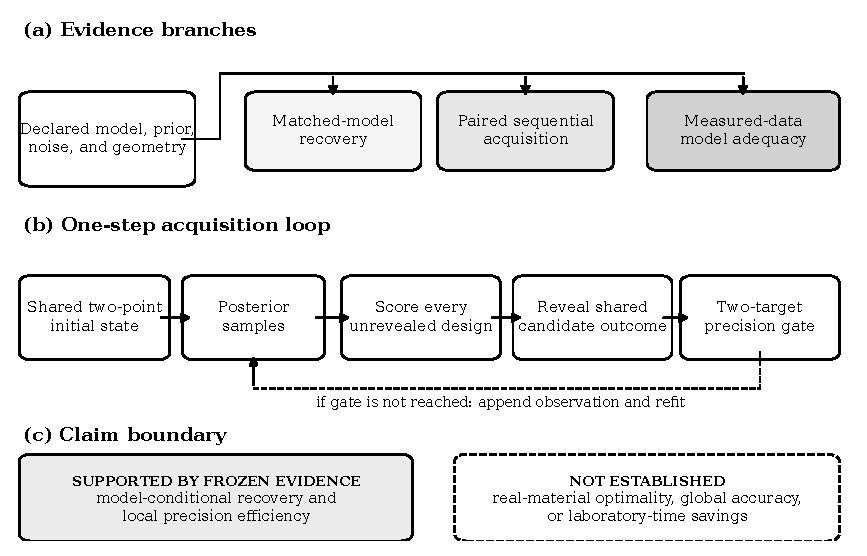
\includegraphics[width=0.98\textwidth]{study_workflow_full.pdf}
  \caption{Study architecture and interpretation boundary. The three evidence
  branches share declared model and data contracts but answer different
  questions. In the sequential branch, every policy begins from the same two
  observations and reveals a pre-generated candidate-indexed outcome. The
  dashed return arrow denotes refitting when the local precision gate is not
  reached. Hatch patterns and line styles are used so the figure remains
  interpretable in grayscale.}
  \label{fig:study-workflow}
\end{figure*}

\section{Research Questions and Evidence Scope}
The study is organized around four research questions. \emph{RQ1} asks whether
the implemented six-coordinate inference problem is locally sensitive in all
active directions and whether the posterior computation can recover known
matched-model parameters. \emph{RQ2} asks whether greedy raw EIG reaches one
declared local precision gate with fewer measurements than the fixed traversal
when both policies see identical candidate outcomes. \emph{RQ3} asks the
corresponding question for EIG per prespecified modeled cost, evaluated by
total modeled acquisition cost rather than count. \emph{RQ4} asks how well the
low-order forward laws describe accepted public measured records in sample.

The evidence ladder in Fig.~\ref{fig:study-workflow} prevents answers from
being combined beyond their design. Local Fisher rank is not global
identifiability; matched-model recovery is not validation on real ferrites;
posterior precision is not truth proximity; and in-sample measured residuals
are not held-out predictive accuracy. The acquisition result is therefore an
algorithmic, model-conditional comparison under a finite library and a local
gate. This explicit estimand is narrower than ``optimal magnetic-component
identification,'' but it is reproducible and falsifiable.

The current frozen evidence reports the three-policy comparison that was run:
raw EIG, EIG divided by modeled cost, and a deterministic fixed
channel-balanced traversal. Randomized balanced, predictive-variance, and
Laplace/D-optimal comparators are implemented in the subsequent protocol but
have no frozen numerical result in this paper. They are consequently discussed
as planned extensions, not as observed outcomes.

\section{Related Work}
\subsection{Magnetic loss and permeability models}
The Steinmetz power law remains a compact engineering description for
sinusoidal loss, while loss-separation and hysteresis models provide more
physical decompositions~\cite{steinmetz1892,bertotti1988,jiles1986}.
Converter waveforms motivated modified and generalized Steinmetz relations
that integrate the instantaneous flux-density trajectory or use waveform
correction factors~\cite{reinert2001,li2001,venkatachalam2002}. Measurement-led
and loss-separation approaches further show why coefficients fitted under one
waveform or operating window need not transfer unchanged to another
~\cite{vandenbossche2004,roshen2007}.
Subsequent work improved practical loss calculation and reviewed the physical
contributions to loss in soft ferrites~\cite{muehlethaler2012,dobak2022}.
Textbook treatments emphasize that material law, geometry, winding, and
thermal assumptions must remain distinct in component design
~\cite{snelling1988,mclyman2011}.

Frequency-dispersive permeability is commonly described through relaxation
or resonance spectra. The Cole--Cole law introduced a broadened relaxation
distribution~\cite{cole1941}; applying its algebraic form to permeability is
an engineering adaptation rather than a claim that ferrite magnetization is a
dielectric process. Classical ferrite dispersion theory and measurements of
Mn--Zn and Ni--Zn ferrites show that
domain-wall motion, rotational processes, resonance, and relaxation can all
shape $\mu'$ and $\mu''$~\cite{snoek1948,tsutaoka2003}. The single-pole model used here
is therefore intentionally diagnostic: a large loss-component residual is
evidence for missing dynamics, not a parameter-estimation failure alone.

Open magnetic datasets now permit reproducible comparisons beyond individual
vendor plots. MagNet provides systematically measured core-loss data across
materials and excitations~\cite{magnet2022}, while the LEA material database
publishes machine-readable permeability and loss records with source
metadata~\cite{materialdatabase}. Public data improve traceability but do not
substitute for a controlled multi-lot characterization campaign.

\subsection{Bayesian calibration and experimental design}
Bayesian calibration represents parameter uncertainty conditional on a
forward model, likelihood, and prior~\cite{gelman2013}. Computer-experiment
literature distinguishes emulator uncertainty, observation error, calibration
parameters, and structural discrepancy~\cite{sacks1989,kennedy2001}.
Validation frameworks consequently compare predictions with observations
rather than treating posterior concentration as proof of physical validity
~\cite{bayarri2007}. Ignoring discrepancy can bias inferred physical
parameters and produce overconfident extrapolation~\cite{brynjarsdottir2014}.
Calibration theory for imperfect simulators also demonstrates that the
physical parameter and discrepancy can be confounded unless additional
structure is imposed~\cite{tuo2015,plumlee2017}. We do not introduce an
unidentified discrepancy process into the present six-parameter fit; instead,
measured residuals are reported as a separate adequacy diagnostic.

Bayesian experimental design formalizes the value of a proposed observation
through expected utility. Lindley's information criterion
~\cite{lindley1956}, foundational reviews~\cite{chaloner1995,ryan2016}, and
classical optimum-design methods~\cite{atkinson2007} motivate the EIG
criterion used here. Estimation remains challenging because the predictive
density is generally unavailable; relevant strategies include Laplace and
MCMC approximations~\cite{ryan2003}, nested Monte Carlo
~\cite{rainforth2018}, multilevel estimators~\cite{goda2020}, stochastic simulation-based optimization
~\cite{huan2013}, and variational bounds~\cite{foster2019}. Adaptive-policy
amortization offers a scalable direction for longer experimental sequences
~\cite{foster2021}, but the present work deliberately uses a transparent
one-step ranking over a finite candidate library.

Information-based acquisition connects Shannon entropy and
Kullback--Leibler divergence to active data selection
~\cite{shannon1948,kullback1951,mackay1992}. Classical D-optimal design instead
optimizes a determinant of an information matrix and is linked to equivalence
theorems~\cite{kiefer1960,atkinson2007}. These criteria coincide only under
particular approximations; the fixed traversal used in the reported benchmark
is neither of them.

\section{Magnetic-Core Models}
\subsection{Core loss}
For sinusoidal excitation within a specified operating window, the Steinmetz
model is
\begin{equation}
  P_v(f,B_{\mathrm{pk}})=k f^{\alpha}B_{\mathrm{pk}}^{\beta},
  \label{eq:steinmetz}
\end{equation}
where $P_v$ is volumetric loss and $(k,\alpha,\beta)$ are inferred parameters
~\cite{steinmetz1892}. The units of $k$ depend on the units used for $P_v$,
$f$, and $B_{\mathrm{pk}}$. Equation~\eqref{eq:steinmetz} is not temperature
dependent in the present implementation. Measured-data analysis therefore
uses a specified temperature subset; extrapolation across temperature is out
of scope. More general waveform-dependent loss equations remain important for
converter application studies~\cite{reinert2001,muehlethaler2012}.

\subsection{Complex permeability}
We adopt the $e^{j2\pi ft}$ time convention and write
$\mu_r=\mu'-j\mu''$, so the reported loss component is
$\mu''=-\operatorname{Im}\mu_r\geq0$ for a passive response. The relative
complex permeability is represented with a single Cole--Cole
relaxation~\cite{cole1941},
\begin{equation}
 \mu_r(f)=1+\frac{\mu_s-1}
 {1+\left(jf/f_{\mathrm{rel}}\right)^{1-a_{\mathrm{cc}}}},
 \label{eq:colecole}
\end{equation}
where $\mu_s$ is low-frequency permeability, $f_{\mathrm{rel}}$ is a
relaxation frequency, and $a_{\mathrm{cc}}$ broadens the relaxation. Storage
and loss components are evaluated separately because a model can fit $\mu'$
while failing to represent $\mu''$. A one-pole model is a deliberate
low-order approximation, not a complete ferrite loss model.

Equation~\eqref{eq:colecole} fixes the high-frequency asymptote to unity and
absorbs the angular-frequency convention into $f_{\mathrm{rel}}$. The real
and loss components follow from the same complex denominator, which prevents
independent tuning of $\mu'$ and $\mu''$. For an optional inductance channel,
the real component is mapped through
$L_m=\mu_0\mu' N^2A_e/\ell_e$ using specified geometry
~\cite{snelling1988,mclyman2011}. Geometry is never inferred jointly with
material parameters in the present study.

\subsection{Validity window}
Both forward laws are isothermal and evaluated only inside specified data
ranges. A data point is defined by channel, frequency, peak flux density, and
temperature. Core-loss points require positive $B_{\mathrm{pk}}$; permeability
points use small-signal records. The likelihood rejects mixed temperature
cohorts. Measured permeability uses material-specific cohorts of
$25\pm0.75\,^{\circ}\mathrm C$ for N87 and $30\pm0.75\,^{\circ}\mathrm C$ for
N95. Measured core loss uses $25\pm0.5\,^{\circ}\mathrm C$ for N49, N87, and
N95, and $100\pm0.5\,^{\circ}\mathrm C$ for 3C95.
These restrictions prevent an apparently precise posterior from silently
extrapolating across temperature, waveform, or excitation regime.

\begin{table*}[t]
\caption{Active parameters, roles, transformations, and principal channels.}
\label{tab:parameters}
\centering\small
\begin{tabular}{@{}lllll@{}}
\toprule
Physical parameter & Active coordinate & Role & Principal response & Main limitation \\
\midrule
$k$ & $\log k$ & core-loss scale & $P_v$ & units follow the declared convention \\
$\alpha$ & $\alpha$ & frequency exponent & $P_v$ & local to sinusoidal, isothermal data \\
$\beta$ & $\beta$ & flux-density exponent & $P_v$ & no waveform or DC-bias dependence \\
$\mu_s$ & $\log\mu_s$ & low-frequency permeability & $\mu',L_m$ & fixed rather than inferred geometry \\
$f_{\mathrm{rel}}$ & $\log f_{\mathrm{rel}}$ & relaxation frequency & $\mu',\mu''$ & one effective relaxation only \\
$a_{\mathrm{cc}}$ & $a_{\mathrm{cc}}$ & relaxation broadening & $\mu',\mu''$ & no multiple resonances \\
\bottomrule
\end{tabular}
\end{table*}

\section{Bayesian Calibration and Design}
Let $\theta=(\log k,\alpha,\beta,\log\mu_s,\log f_{\mathrm{rel}},
a_{\mathrm{cc}})$ denote the active transformed parameters. Log coordinates
enforce positivity of scale parameters while retaining direct coordinates for
the exponents. For observation
$y_o$ at design $d_o$, the likelihood is
\begin{equation}
 p(\mathbf y\mid\theta,\mathbf d)=
 \prod_o \mathcal N\!\left(y_o;F_o(\theta,d_o),\sigma_o^2\right),
\end{equation}
with fixed relative scales. Synthetic scales are 3% for core loss, 2% for
$\mu'$, 5% for $\mu''$, and 1% for inductance; measured records use a 3%
relative scale as a weighting model. The posterior is
\begin{equation}
 p(\theta\mid\mathbf y,\mathbf d)\propto
 p(\mathbf y\mid\theta,\mathbf d)p(\theta).
\end{equation}
Priors are defined directly in the transformed space used by the sampler, so
no inverse-transform Jacobian is added to this active-coordinate density.
Bounds encode physically admissible numerical domains, not empirical proof
that the chosen model is correct.

The six coordinates divide into two response blocks in the likelihood but are
sampled jointly. Core-loss observations directly update
$(\log k,\alpha,\beta)$, while permeability and inductance observations update
$(\log\mu_s,\log f_{\mathrm{rel}},a_{\mathrm{cc}})$. Joint sampling retains a
single posterior contract and permits one acquisition library to contain all
channels; it does not create physical coupling absent from the forward laws.
Table~\ref{tab:parameters} makes this structural separation explicit.

Four uncertainty sources must be distinguished. \emph{Parameter uncertainty}
is represented by posterior draws conditional on the chosen model and fixed
geometry. \emph{Observation uncertainty} enters through the declared Gaussian
scale. \emph{Monte Carlo uncertainty} arises because posterior and EIG
integrals are approximated by finite samples. \emph{Structural uncertainty}
is exposed by measured residuals but is not parameterized in the likelihood.
Only the first three are quantified in parts of the present workflow; an EIG
score interval is therefore not a total physical-uncertainty interval.

\subsection{Posterior computation and diagnostics}
Posterior sampling uses the affine-invariant ensemble construction
~\cite{goodman2010} implemented by \texttt{emcee}~\cite{foreman2013}. Each
ensemble retains 5000 steps after 1000 warm-up steps for each
of 48 walkers. Initial states are perturbations of the prior center and both
initialization and proposal streams are deterministically seeded. A fit is
accepted only with finite integrated autocorrelation estimates, at least 50
retained steps per autocorrelation time, effective sample size at least 400,
mean acceptance between 0.20 and 0.60, and finite log probability for every
retained sample.

These checks follow the principle of comparing Monte Carlo variation with
between-sequence behavior~\cite{gelman1992} and modern effective-sample-size
practice~\cite{vehtari2021}, but interacting ensemble walkers are not treated
as independent chains. Accordingly, the paper does not report a conventional
$\widehat R$ for the ensemble. Diagnostic failure invalidates a measured fit
for quantitative publication rather than being repaired by discarding an
unfavorable seed.

Matched-model recovery also exercises the complete forward--likelihood--
sampler--summary path against known generating values. It is an implementation
check related to posterior-quantile validation~\cite{cook2006}, but five
independent fits do not constitute simulation-based calibration
~\cite{talts2018}. A calibrated rank experiment would require many more
prior-predictive replications and a uniform-rank diagnostic. Posterior and
residual graphics are interpreted as part of a Bayesian workflow rather than
as substitutes for numerical diagnostics~\cite{gelman1996,gabry2019}.

The local Fisher approximation~\cite{fisher1922} is
\begin{equation}
 \mathcal I_{ij}=\sum_o\frac{1}{\sigma_o^2}
 \frac{\partial F_o}{\partial\theta_i}
 \frac{\partial F_o}{\partial\theta_j}.
\end{equation}
Its spectrum is computed over the exact active vector and with reported
scaling. A large condition number indicates locally sloppy combinations but
does not by itself establish global non-identifiability~\cite{gutenkunst2007}.
Geometric analyses of sloppy models likewise interpret broad eigenvalue
spectra as anisotropic distinguishability, not as a universal parameter
ranking~\cite{transtrum2015}. The spectrum is therefore reported together
with its dimension and scaling convention.

Let $\mathcal D_t=(\mathbf y_t,\mathbf d_t)$ denote the observations available
before acquisition step $t$. For candidate $d$, the one-step EIG is
the conditional mutual information~\cite{lindley1956,chaloner1995}
\begin{equation}
 \mathrm{EIG}_t(d)=
 \mathbb E_{\substack{\theta\sim p(\theta\mid\mathcal D_t)\\
 y\sim p(y\mid\theta,d)}}
 \left[
 \log p(y\mid\theta,d)-\log p(y\mid d,\mathcal D_t)
 \right],
 \label{eq:eig}
\end{equation}
where
\begin{equation}
 p(y\mid d,\mathcal D_t)=
 \int p(y\mid\vartheta,d)
 p(\vartheta\mid\mathcal D_t)\,d\vartheta .
\end{equation}
For outer draws $(\theta_i,y_i)$ and inner posterior draws $\vartheta_{ij}$,
the implemented nested estimator is
\begin{equation}
 \begin{aligned}
 \widehat U(d)=\frac{1}{N}\sum_{i=1}^{N}\bigg[&
 \log p(y_i\mid\theta_i,d)\\[-0.2ex]
 &-\log\!\left\{\frac{1}{M}\sum_{j=1}^{M}
 p(y_i\mid\vartheta_{ij},d)\right\}\bigg].
 \end{aligned}
 \label{eq:nmc}
\end{equation}
Finite inner budgets introduce bias through the logarithm and finite outer
budgets introduce variance; close candidates can therefore exchange rank
~\cite{rainforth2018,goda2020}. The convergence campaign described below
tests ranking and downstream endpoint stability rather than assuming one
budget is sufficient.

The reported estimator draws \EIGOuter{} outer parameter--observation pairs
and uses \EIGInner{} inner posterior draws to approximate the posterior-predictive
density~\cite{ryan2003,rainforth2018}. Each score is repeated
\EIGReplicates{} times;
the mean, standard error, 95\% Monte Carlo interval, and top-rank frequency are
retained. Candidate streams are seeded from a stable key comprising channel,
frequency, flux density, and temperature, so list permutation cannot change a
design's draws. We evaluate two distinct objectives: raw EIG for the measurement-count endpoint
and EIG divided by a prespecified modeled acquisition cost for the total-cost
endpoint. These intervals quantify repeated nested-Monte-Carlo variability
conditional on the retained posterior draws and model; they exclude
chain-to-chain, structural-model, geometry, and noise-model uncertainty.

\subsection{Paired sequential policy}
After the same two initial observations---$P_v$ at 30 kHz, 0.05 T, and
$25\,^{\circ}\mathrm C$, and $\mu'$ at 10 kHz and $25\,^{\circ}\mathrm C$---each
policy selects one unrevealed candidate, receives its pre-generated noisy
outcome, refits the posterior, and checks the common precision gate. Raw EIG
maximizes estimated information, EIG/cost maximizes information per modeled
cost, and the comparator follows a deterministic fixed channel-balanced grid
traversal. It is not uniform random sampling, a space-filling design, or a
D-optimal design. All policies share the candidate library, latent truth,
candidate-indexed noisy outcomes, maximum budget, and stopping rule. The
candidate library is isothermal, so it contains no temperature-only duplicates
of the implemented forward laws.
The numerical settings are summarized in Table~\ref{tab:protocol}.

The stopping statistic is the half-width of the central 90\% posterior interval
for the noise-free latent mean response divided by the absolute posterior
median. Observation noise is not added to this gate. The two fixed targets are
$P_v(100\,\mathrm{kHz},0.1\,\mathrm T,25\,^{\circ}\mathrm C)$ at 8\% and
$L_m(100\,\mathrm{kHz},25\,^{\circ}\mathrm C)$ at 5\%. This is a local precision
criterion: it checks neither truth proximity, six-parameter recovery, other
channels, held-out performance, nor model adequacy. A policy that misses either
threshold is recorded as a failure at the maximum budget. Candidate EIG
integrates over the joint six-parameter posterior; only the stopping and
evaluation endpoint is restricted to these two responses.

\begin{table*}[t]
\caption{Finite synthetic acquisition library and declared channel assumptions.}
\label{tab:candidate-library}
\centering\small
\begin{tabular}{@{}llllll@{}}
\toprule
Channel & Frequencies (kHz) & $B_{\mathrm{pk}}$ (T) & Points & Relative noise & Modeled cost \\
\midrule
$P_v$ & 30, 50, 100, 200, 300, 500 & 0.05, 0.10, 0.20 & 18 & 3\% & 60 \\
$\mu'$ & 10, 30, 100, 300, 500, 1000, 2000, 3000 & 0 & 8 & 2\% & 20 \\
$\mu''$ & 10, 30, 100, 300, 500, 1000, 2000, 3000 & 0 & 8 & 5\% & 20 \\
$L_m$ & 10, 100, 1000 & 0 & 3 & 1\% & 15 \\
\bottomrule
\end{tabular}
\begin{minipage}{0.96\textwidth}\footnotesize
All 37 candidates are at $25\,^{\circ}\mathrm C$. Modeled costs are positive
prespecified units used only for the EIG/cost endpoint; they are not measured
instrument or laboratory durations. The two initial observations belong to
the same library and count toward the stopping total.
\end{minipage}
\end{table*}

\section{Computational Reproducibility}
All experiments use fixed software versions, specified model and inference
settings, explicit data selections, and deterministic random seeds. Results
are retained at the individual-seed level and are accepted for aggregation
only when all prespecified validity gates pass.

\begin{table}[t]
\caption{Computational settings used for the reported experiments.}
\label{tab:protocol}
\centering\footnotesize
\begin{tabular}{@{}p{0.32\columnwidth}p{0.62\columnwidth}@{}}
\toprule Item & Setting \\
\midrule
Ensemble sampler & 48 walkers; 1000 warm-up + 5000 retained \\
Convergence criteria & ESS $\geq400$; steps/$\tau\geq50$ \\
Acceptance criterion & $0.20$--$0.60$ \\
Nested EIG & \EIGOuter{} outer; \EIGInner{} inner; \EIGReplicates{} score replicates \\
Sequential budget & at most 25 measurements \\
Acquisition endpoints & raw EIG/count; EIG/cost/modeled cost \\
Temperature cohorts & material and channel specific, as stated in text \\
Precision gate & latent mean response: 8\% $P_v$; 5\% $L_m$ \\
\bottomrule
\end{tabular}
\end{table}

The analysis checks all required seed and material cases before forming
aggregate summaries. Records with nonfinite values, failed convergence, or
boundary-active parameters are excluded according to criteria specified
before evaluation. Numerical statements, tables, and figures are generated
programmatically from the same complete set of accepted records, avoiding
manual transcription or selective replacement of outcomes.

\subsection{Estimator-budget qualification}
The nested estimator was qualified before the 30-seed acquisition campaign.
Twelve posterior states were formed from four seeds (7100--7103) after 2, 4,
and 6 observations. At each state, 27 candidate settings crossed outer budgets
$\{100,300,900\}$, inner budgets $\{50,100,300\}$, and replicate counts
$\{5,10,20\}$. Every setting was compared with a 1200-outer, 400-inner,
40-replicate reference. Two sentinel states were additionally recomputed at
2400 outer and 800 inner draws with 40 replicates. Prefix-nested random streams
made the lower-budget samples literal prefixes of the larger calculations,
reducing irrelevant differences between settings.

The acceptance decision combined the stable top candidate, Spearman rank
correlation, score-interval overlap, relative reference regret, and exact
agreement of downstream count and modeled-cost endpoints. Ten disjoint seeds
(7200--7209) supplied that downstream check. The selected setting was then
locked before the confirmatory acquisition seeds 7300--7329 were evaluated.
This separation prevents selecting an estimator budget because it happened to
produce the most favorable headline comparison.

\begin{table*}[t]
\caption{Evidence layers retained for the current frozen release.}
\label{tab:evidence-layers}
\centering\footnotesize
\begin{tabular}{@{}p{0.17\textwidth}p{0.22\textwidth}p{0.32\textwidth}p{0.20\textwidth}@{}}
\toprule
Layer & Prespecified cases & Retained public evidence & Scientific role \\
\midrule
Matched recovery & 5 generating seeds & seed-level parameter summaries & implementation check \\
Estimator states & $4\times3=12$ & state records and flattened posterior samples & budget qualification \\
Estimator grid & 27 budget combinations across 12 states & 108 candidate-score records plus 12 references & ranking stability \\
Doubled-budget audit & 2 sentinel states & 2 doubled-budget score records & reference sensitivity \\
Downstream validation & 10 seeds & 10 policy endpoint records & endpoint stability \\
Confirmatory acquisition & 30 paired seeds & 30 complete policy trajectories & count and cost endpoints \\
Measured adequacy & declared material/source pairs & aggregate metrics and disclosed exclusions & model discrepancy diagnostic \\
\bottomrule
\end{tabular}
\end{table*}

The public audit projection retains the campaign records needed to reconstruct
the acquisition endpoints and estimator decision while removing machine paths
and scheduler metadata. Posterior arrays are retained flattened over sampling
draws; because walker and iteration indices are not present, they are not
described as raw MCMC chains. The compact frozen summary authenticates the
reported measured-fit aggregates and exclusions, but the audit projection does
not independently reconstruct those fits. Raw upstream measured curves remain
governed by their source repositories and are not redistributed here.

\section{Evaluation Protocol}
Five fixed seeds are used for matched-model recovery. A disjoint, prespecified
set of \EIGSeedCount{} seeds is used for the paired acquisition comparison only
after the nested-Monte-Carlo setting passes a separate convergence study.
That study uses prefix-nested common random numbers and a deterministic paired
bootstrap of the replicate-mean selector; it requires stable candidate and
reference winners, rank correlation, score-interval overlap, low reference
regret, and downstream endpoint agreement. The policies share initial observations,
candidate library, realized candidate outcomes, noise policy, budget, and stopping
rule. Results include per-seed counts, modeled costs, and failures, not only
an aggregate ratio. The stopping rule concerns posterior precision
of two latent mean responses and is not an accuracy or coverage guarantee.

For recovery, observations are generated from the same six-parameter forward
family used in inference. A parameter vector is drawn independently for each
seed from a datasheet prior fixed before that draw; the prior is never rebuilt
from the realized truth. Sampler walkers are initialized around the fixed
prior center, not around the hidden generating vector. Observation noise is
then generated independently. This is a prior-predictive matched-model design:
it removes oracle centering while retaining favorable equality between the
data-generating and inference model families. The reported error is the absolute
relative difference between posterior median and the generating value. The
interval statistic counts whether that value falls within the equal-tailed
90\% model-conditional posterior credible interval. With only five seeds, the
count is a descriptive implementation check, not a coverage experiment.
The Fisher matrix is evaluated in the exact transformed coordinate system used
by sampling.

For the paired acquisition analysis, a stable design-keyed seed generates one
noisy observation for every candidate before any policy is run. A policy
reveals the already generated value when it selects that design. Thus policy
order cannot change the noise attached to a candidate, and all policies in a
seed share the same latent truth and candidate outcome map. The 30 paired
differences are the unit of analysis. Descriptive means, medians, standard
deviations, win and failure rates, and percentile intervals are computed from
those differences. The reported confidence interval uses 10,000 deterministic
paired bootstrap resamples. It quantifies between-seed variation in this
matched-model experiment and is not a population-wide material claim.

The measured evaluation uses public complex-permeability curves for specified
N95, N87, and 3C95 source/material pairs and datasheet core-loss curves for
N49, N87, N95, and 3C95~\cite{materialdatabase}. Input-data versions,
temperature cohorts, unit conversions, and range filters were fixed before
inference. Storage/loss permeability errors, core-loss residuals, boundary
activity, and operating-window coverage are reported separately. Records with
failed convergence or active boundary flags are retained for diagnostic review
but excluded from aggregate numerical claims.

Core-loss adequacy is summarized by in-sample relative root-mean-square error
(RRMSE) within each temperature cohort. Permeability adequacy is evaluated
separately for storage and loss components because combining them can conceal
a poor $\mu''$ fit behind the larger magnitude of $\mu'$. These metrics assess
the selected low-order model on observed records; they are neither held-out
prediction errors nor component-level thermal validation.

\section{Results}

\subsection{Identifiability and synthetic recovery}
The synthetic $6\times6$ Fisher matrix was full rank. As shown in
Fig.~\ref{fig:synthetic-results}(a), its eigenvalues span
\scientific{\FisherMin} to \scientific{\FisherMax}, giving a full-matrix
condition number of \scientific{\FisherCondition}.
The broad spectrum indicates strong local sensitivity anisotropy in the active
transformed coordinates; it does not establish global identifiability.
Fig.~\ref{fig:synthetic-results}(b) shows the absolute posterior-median
errors for each parameter and seed. Across five prior-predictive matched-model
data sets, the per-parameter medians range from \RecoveryMedianMin\% to
\RecoveryMedianMax\%. The known values fell within \RecoveryInclusion{}
equal-tailed 90\% model-conditional posterior credible intervals. This
observed inclusion count is descriptive, not a coverage estimate.
Table~\ref{tab:recovery} reports the same matched-model recovery check.

% Generated from immutable release candidate 20260812T035654Z_a0703698ace9; do not edit.
\begin{table}[t]
\caption{Matched-model recovery and inclusion of the generating value in equal-tailed 90\% posterior credible intervals (five synthetic seeds).}
\label{tab:recovery}
\centering\small
\begin{tabular}{lrr}
\toprule Parameter & Median error (\%) & Truth included \\
\midrule
$k$ & 5.85 & 4/5 \\
$\alpha$ & 0.27 & 4/5 \\
$\beta$ & 0.36 & 5/5 \\
$\mu_s$ & 0.38 & 5/5 \\
$f_{\mathrm{rel}}$ & 0.87 & 5/5 \\
$a_{\mathrm{cc}}$ & 0.62 & 5/5 \\
\bottomrule
\end{tabular}
\end{table}


\begin{figure*}[t]
  \centering
  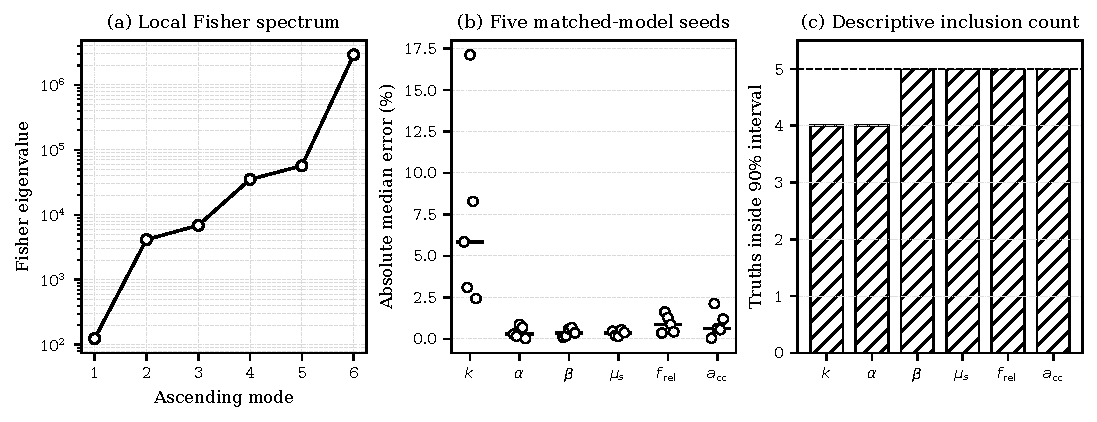
\includegraphics[width=\textwidth]{synthetic_diagnostics_full.pdf}
  \caption{Synthetic local identifiability and matched-model recovery. (a)
  Fisher eigenvalues in ascending order. (b) Absolute posterior-median errors
  across five seeds; circles are horizontally
  offset for visibility and horizontal ticks mark medians. (c) Number of the
  five generating values inside each equal-tailed 90\% model-conditional
  posterior interval. The five-seed inclusion count is descriptive and is not
  a coverage estimate.}
  \label{fig:synthetic-results}
\end{figure*}

\subsection{Nested-estimator qualification}
The conservative reference setting of 1200 outer draws, 400 inner draws, and
40 score replicates was selected by the prespecified convergence decision.
The doubled-budget sentinels preserved the required selector behavior, and the
ten downstream validation seeds preserved both count and modeled-cost
endpoints. This result qualifies the numerical setting for the subsequent
campaign; it does not make each finite EIG score exact. In particular, the
reported score intervals remain conditional on the retained posterior and
forward model.

\subsection{Paired synthetic acquisition}
Fig.~\ref{fig:acquisition-results} makes the paired outcome structure
explicit. Raw EIG reached the two-target latent mean-response precision gate
with \EIGRange{} measurements, while the fixed channel-balanced grid traversal
required \UniformRange{}. Raw EIG used fewer measurements in every paired run,
with a mean reduction of \EIGReduction\%. These results evaluate selection
efficiency for the count endpoint in this \EIGSeedCount-seed matched-model
experiment. The mean paired count difference has a bootstrap 95\% interval of
\EIGCountDifferenceCILow--\EIGCountDifferenceCIHigh{} measurements; the paired
win rate is \EIGCountWinRate\% and the raw-EIG gate-failure rate is
\EIGRawFailureRate\%.
The seed-level distribution is concentrated rather than hidden by the mean:
29 pairs favor raw EIG by four measurements and one pair favors it by five.
\ifdefined\EIGCostReduction
For the separate modeled-cost endpoint, EIG/cost gave a descriptive mean paired
reduction of \EIGCostReduction\%; neither policy comparison had a gate failure.
The cost units are prespecified rather than measured laboratory time.
\else
EIG/cost is evaluated separately against total modeled acquisition cost; no
claim of measured laboratory-time savings is made.
\fi

\begin{figure*}[t]
  \centering
  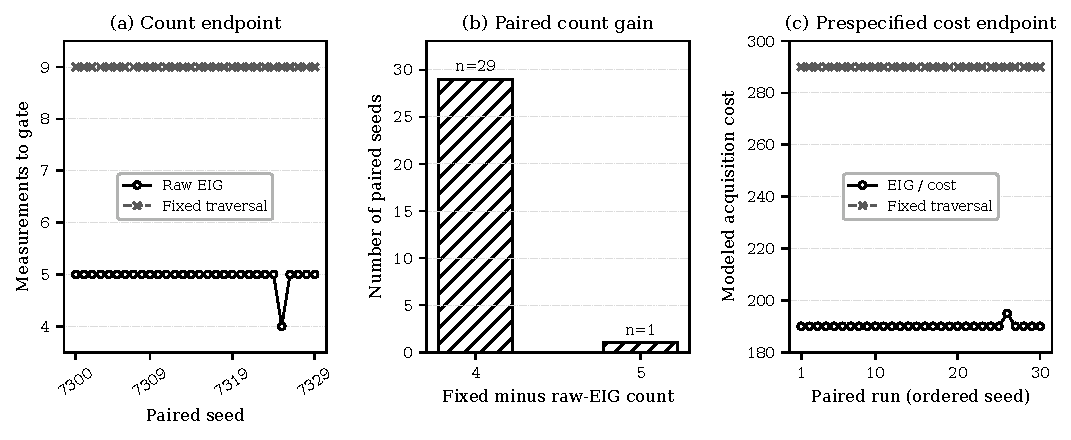
\includegraphics[width=\textwidth]{acquisition_diagnostics_full.pdf}
  \caption{Thirty-seed paired matched-model acquisition results. (a) Raw-EIG
  and fixed-traversal measurement counts at the common two-target precision
  gate. (b) Distribution of paired count gains, defined as fixed minus raw
  EIG. (c) Total prespecified modeled cost for EIG/cost and the fixed traversal.
  Candidate-indexed outcomes are identical across policies within each seed;
  modeled cost is an assumed endpoint, not observed laboratory duration.}
  \label{fig:acquisition-results}
\end{figure*}

\subsection{Measured-data model adequacy}
Fig.~\ref{fig:measured-results} compares the in-sample relative
root-mean-square errors (RRMSEs) of the accepted measured-data fits. For
LEA Material Database permeability records that satisfied the convergence
criteria, RRMSEs were
\NEightySevenMuRealRms\%/\NEightySevenMuImagRms\% for
$\mu'/\mu''$ on N87 and \NNinetyFiveMuRealRms\%/\NNinetyFiveMuImagRms\% on
N95. The larger $\mu''$ errors expose discrepancy in the one-pole model.
N87 and 3C95 MagNet records failed convergence or boundary gates and were
excluded from numerical claims~\cite{magnet2022}. Measured Steinmetz fits
produced in-sample RRMSEs of \NEightySevenPcvRms\% (N87), \NFortyNinePcvRms\%
(N49), \ThreeCNinetyFivePcvRms\% (3C95), and \NNinetyFivePcvRms\% (N95)
within their specified temperature cohorts. These are fit residuals, not
held-out errors.

\begin{figure*}[t]
  \centering
  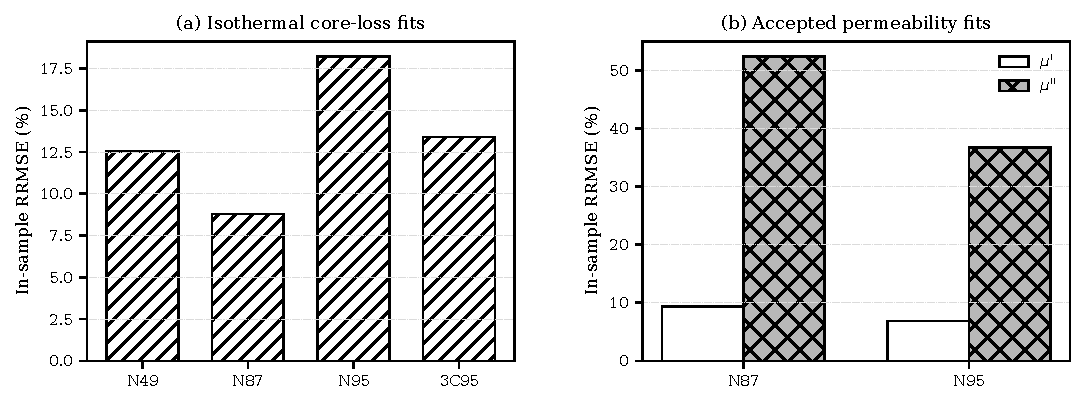
\includegraphics[width=\textwidth]{measured_adequacy_full.pdf}
  \caption{Measured-data in-sample model adequacy for accepted fits. (a)
  Isothermal Steinmetz core-loss RRMSE. (b) Separate storage and loss
  permeability RRMSE for accepted LEA records. The much larger $\mu''$ error
  is not absorbed into a combined complex-valued metric. Convergence-invalid
  or boundary-active MagNet fits are excluded from these numerical bars and
  disclosed in the text.}
  \label{fig:measured-results}
\end{figure*}

All numerical results in this section, including
Figs.~\ref{fig:synthetic-results}, \ref{fig:acquisition-results},
and~\ref{fig:measured-results}, use the
same prespecified models, data filters, random seeds, and evaluation criteria.

\section{Discussion and Limitations}
\subsection{Interpretation of the evidence}
The framework separates whether available measurements constrain parameters
within a chosen model from whether that model represents measured material
behavior. Fisher information and posterior width address the former locally
or conditionally; reported in-sample residuals expose, but do not fully
quantify, the latter. Held-out predictive validation remains future work.

The synthetic results support implementation-level conclusions. Full local
rank shows that every active coordinate affects the specified synthetic
experiment, while the broad spectrum shows that those effects occur at very
different scales. The recovery table then checks the nonlinear posterior under
matched truth. Neither result implies that the same coordinates are uniquely
physical when the material response lies outside the six-parameter family.
This distinction matters for converter models because several parameter sets
can produce similar loss or permeability over a narrow operating window yet
diverge when frequency, flux density, or temperature changes.

The paired acquisition result shows that raw EIG exploited posterior structure
in the matched problem: it reached the two-target precision gate with fewer
measurements for every reported seed under shared candidate outcomes. The
result means only that fewer measurements were needed to narrow two specified
latent mean-response intervals. It does not establish accurate recovery of the
magnetic component, global predictive accuracy, or robustness to model
misspecification.

\subsection{Implications for converter modeling}
For a converter workflow, the posterior is most useful as a conditional input
to loss, inductance, and sensitivity calculations over the specified
operating region. Posterior draws can be propagated through a component model
instead of substituting one nominal coefficient set, allowing a designer to
determine whether parameter uncertainty materially affects thermal or magnetic
design margins. The Fisher spectrum can motivate testing whether a new channel
or a wider, physically controlled excitation range would constrain a weak
direction more effectively than densifying the original sweep
~\cite{chaloner1995,atkinson2007}.

Measured residuals define a separate model-adequacy assessment. The accepted core-loss
fits show the error remaining after estimating Steinmetz coefficients inside
one temperature cohort. The much larger loss-component permeability residuals
show that a single Cole--Cole pole cannot be treated as a broadband physical
description for these records. A component calculation that is sensitive to
$\mu''$ should therefore retain an explicit discrepancy allowance or adopt a
higher-order permeability law before relying on posterior parameter width.
Conversely, a reasonable $\mu'$ residual does not validate $\mu''$, because
the two components occupy different numerical scales and correspond to
different design consequences.

The common evaluation protocol safeguards this interpretation by preventing
combination of a favorable recovery run, a figure from another seed set, and
a measured fit produced under different filters. Fixed model settings, data
selections, and random seeds also make it possible to distinguish sampling
variation from changes to the computational experiment.

\subsection{Threats to validity}
Internal validity is limited by five synthetic recovery seeds and
\EIGSeedCount{} paired acquisition seeds. Pairing controls differences in
candidate outcomes between policies. A prespecified convergence study compares
candidate ranks and downstream endpoints against a higher-budget reference;
finite nested Monte Carlo variance nevertheless remains. Synthetic recovery is
matched-model, and the observed interval-inclusion count is too small to
establish calibrated coverage.

The policy comparison is against one fixed channel-balanced traversal; it
does not establish dominance over randomized balanced, predictive-variance,
Fisher-greedy, or D-optimal designs. Observation noise and geometry are fixed,
and estimator intervals are not total physical-uncertainty intervals.

Construct validity is limited by the low-order forward models and available
data. The Steinmetz relation is temperature independent, and one Cole--Cole
pole does not capture all ferrite relaxation, resonance, or loss processes
~\cite{tsutaoka2003}. Measured errors are in-sample. Public curves may also
contain digitization, instrument, preprocessing, and source-specific errors
not represented by the likelihood. Excluding convergence-invalid or
boundary-active records prevents unsupported aggregate claims but restricts
the population represented by the accepted subset.

External validity is confined to the specified channels, temperature cohorts,
excitation ranges, materials, and cost model. The measured-data EIG ranking is
a model-conditional acquisition suggestion, not a validated optimal laboratory
plan, particularly given the observed $\mu''$ discrepancy. Measurement-count reductions
must not be interpreted as laboratory-time savings because setup, settling,
calibration, rejection, and batch costs were not measured. The results do not
replace held-out validation, controlled multi-lot characterization,
switching-waveform experiments, or component qualification. Those extensions
require new experimental evidence rather than broader interpretation of the
present results.

\subsection{Evidence required for broader claims}
Three additions would materially change the evidential scope. First, a new
checksum-locked paired campaign must compare EIG with randomized balanced,
predictive-variance, and Fisher/Laplace D-optimal policies under the same
outcome table, count budget, and cost table. The implemented follow-on protocol
declares these methods but the current release contains no outcome from it.
Second, a disjoint latent-response grid must test truth error and interval
inclusion away from both acquisition candidates and stopping targets. Such a
test can detect a narrow-but-wrong matched-model posterior, although it still
cannot diagnose structural discrepancy. Third, a laboratory study needs
independently calibrated noise, measured acquisition durations, multiple lots,
and held-out temperature/frequency/flux regions. Only that third layer could
support claims about real-material measurement or time savings.

This hierarchy also defines negative results that would revise the conclusion:
unstable EIG rankings under increased Monte Carlo budgets, loss against stronger
paired comparators, poor disjoint-grid prediction despite reaching the gate,
or failure of real-data residual and coverage criteria. Publishing these
decision boundaries makes the present positive result testable rather than
open ended.

\section{Conclusion}
Bayesian calibration recovered the six active Steinmetz and Cole--Cole
parameters with per-parameter median absolute relative errors of
\RecoveryMedianMin\%--\RecoveryMedianMax\% across five matched-model synthetic
data sets. The known values fell within \RecoveryInclusion{} equal-tailed
90\% model-conditional posterior credible intervals. Under paired candidate
outcomes and a common stopping rule, raw EIG reached the two-target latent
mean-response precision gate with \EIGRange{} measurements, compared with
\UniformRange{} for the fixed channel-balanced grid traversal, a descriptive
mean reduction of \EIGReduction\% across \EIGSeedCount{} seeds. The paired
count-difference bootstrap interval was \EIGCountDifferenceCILow--
\EIGCountDifferenceCIHigh{} measurements, with \EIGCountWinRate\% paired wins
and a \EIGRawFailureRate\% raw-EIG gate-failure rate. The
accepted measured records produced substantially larger RRMSEs for $\mu''$
than for $\mu'$, showing that posterior concentration cannot compensate for an
inadequate permeability law. The workflow links inference, local
identifiability, measurement selection,
model-adequacy checks, and traceable evidence within the tested models,
public data records, and operating ranges.

\appendix
\section{Exact Sequential Evaluation Logic}
For each confirmatory seed, the synthetic truth is drawn once from the fixed
prior. One outcome per exact candidate identity is then generated and stored.
Each policy is evaluated by the following logic:

\begin{enumerate}
  \item Start with the same declared $P_v$ and $\mu'$ observations.
  \item Fit the six-coordinate posterior and require all sampler gates.
  \item If both target intervals satisfy the precision gate, retain count and
        modeled cost and stop successfully.
  \item Otherwise score or traverse only unrevealed candidates. Raw EIG uses
        $\widehat U(d)$; EIG/cost uses $\widehat U(d)/c(d)$; the fixed policy
        uses its deterministic channel-balanced order.
  \item Break deterministic ties by exact design identity, reveal the stored
        outcome for the selected identity, append it, and return to step 2.
  \item If the 25-measurement budget is exhausted, retain the trajectory as a
        failure rather than imputing a stopping count.
\end{enumerate}

This logic separates three random objects: the prior-predictive truth, the
candidate-indexed outcome table, and the policy's numerical scoring stream.
Changing policy order changes neither the truth nor any candidate outcome.
Stable design identities also make EIG scores invariant to permutation of the
input library.

\section{Endpoint and Uncertainty Definitions}
For a latent target $g(\theta)$, the reported precision statistic is
\begin{equation}
 h_g=100\,\frac{q_{0.95}[g(\theta)]-q_{0.05}[g(\theta)]}
 {2\,|q_{0.50}[g(\theta)]|}.
\end{equation}
The gate requires $h_{P_v}\leq8$ and $h_{L_m}\leq5$. The measurement-count
endpoint is the number of revealed observations, including the two initial
points, at the first satisfied gate. The cost endpoint is the sum of declared
channel costs through that same step. Because the cost constants were not
measured, the endpoint is dimensionless modeled burden even though the
configuration names them as seconds for engineering convenience.

For paired seed $s$, count gain is
$\Delta_s=n_{\mathrm{fixed},s}-n_{\mathrm{rawEIG},s}$; modeled-cost gain is
defined analogously for EIG/cost. Resampling is performed over complete paired
seeds, never over unpaired policy outcomes. Monte Carlo score intervals come
from repeated estimates of Eq.~\eqref{eq:nmc}; posterior intervals come from
retained sampler draws; paired bootstrap intervals come from the 30 seed-level
differences. These three intervals answer different questions and are not
interchangeable.

\section{Evidence, Software, and Version Boundary}
The current manuscript is tied to frozen release
\texttt{20260812T035654Z\_a0703698ace9} through a machine-readable result lock.
Generated tables, macros, figures, and the summary are checksum verified before
paper compilation. A separate sanitized audit asset contains the 30 policy
trajectories, estimator states and scores, downstream validation records, and
retained flattened posterior matrices needed to reconstruct the acquisition
and estimator-selection claims. Its scope and digest are recorded in the
repository. Raw measured curves are obtained from the cited upstream sources
and are not redistributed as if they were produced by this study.

The six-page conference snapshot is an immutable historical record associated
with its own earlier release and claim ledger. This full current version keeps
the same A4 two-column visual convention but has no page ceiling, includes the
30-seed confirmatory evidence and estimator qualification, and must not be
used to retroactively reinterpret the snapshot. Source, protocols, result
locks, and verification commands are available in the accompanying public
repository.

\let\standardthebibliography\thebibliography
\renewcommand{\thebibliography}[1]{%
  \standardthebibliography{#1}%
  \setlength{\itemsep}{0pt}%
  \setlength{\parskip}{0pt}%
}
{\fontsize{8}{8.5}\selectfont
\bibliographystyle{ieeetr}
\bibliography{refs}
}
\end{document}
